\documentclass{standalone}

\usepackage{tikz}
\tikzset{chessboard/.style={thick}}%

\begin{document}
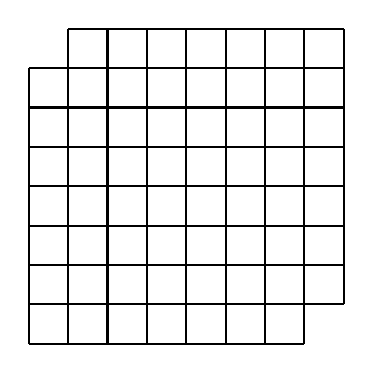
\begin{tikzpicture}[scale=0.5]
  \newif\iffirstdiag          % Switch to control which corners are ommitted.
  \firstdiagtrue              % (flip the switch here)
  %
  \pgfmathtruncatemacro\N{8}  % number of rows/columns
  \pgfmathtruncatemacro\Nmone{\N-1}
  %
  % draw internal lines
  \foreach \i in {1,2,...,\Nmone}
  {
    \draw[chessboard] (0,\i) -- (\N,\i);  % We control the horizontals...
    \draw[chessboard] (\i,0) -- (\i,\N);  % ...and the verticals.
                                          % We can deluge you with a thousand
                                          % channels or expand one single
                                          % image to crystal clarity and 
                                          % beyond...
  }
  %
  % draw external lines
  \iffirstdiag
    \draw[chessboard] (0,0)  -- (\Nmone,0);    % bottom
    \draw[chessboard] (1,\N) -- (\N,\N);       % top
    \draw[chessboard] (0,0)  -- (0,\Nmone);    % left
    \draw[chessboard] (\N,1) -- (\N,\N);       % right
  \else
    \draw[chessboard] (1,0)  -- (\N,0);        % bottom
    \draw[chessboard] (0,\N) -- (\Nmone,\N);   % top
    \draw[chessboard] (0,1)  -- (0,\N);        % left
    \draw[chessboard] (\N,0)  -- (\N,\Nmone);  % right
  \fi
\end{tikzpicture}
\end{document}
